\subsection*{Appendix A.2}
\begin{equation}
    P_1x_1+p_2x_2 = y
\end{equation}
Where $P_1$ and $P_2$ are the prices of good 1 and good 2 respectively. $x_1$ and $x_2$ are the quantities of good 1 and good 2 respectively. $y$ is the income.\\
If you plot this, the slope is $-\frac{P_1}{P_2}$. This is the budget constraint. Operating within the budget constraint is inefficient, outside is unobtainable. 
\begin{figure}[H]
    \centering
    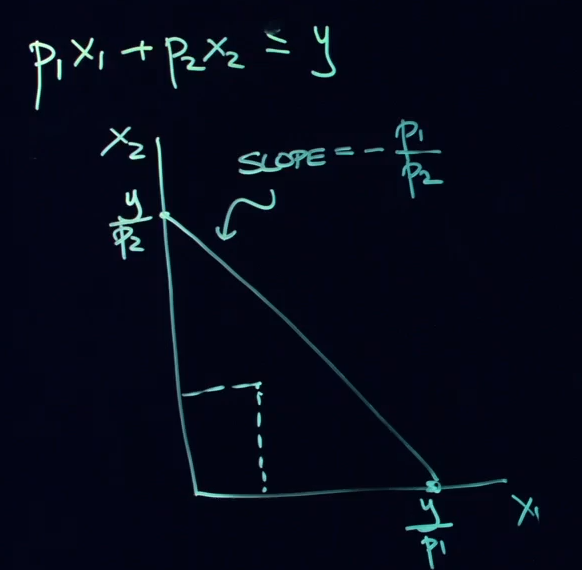
\includegraphics[width=0.5\textwidth]{Chapter6/BudgetConstraint.png}
    \caption{Budget Constraint}
    \label{fig:Budget_Constraint}
\end{figure}
We can combine the constraint with the indifference curve to find the optimal point.\\
There will be some indifference curve with only one point on the budget constraint. This is the optimal point.\\
Where the marginal rate of substitution is equal to the slope of the budget constraint.
\begin{figure}[H]
    \centering
    
\includegraphics[width=0.5\textwidth]{Chapter6/IndifferenceCurveBudgetConstraint.png}
    \caption{Indifference Curve and Budget Constraint}
    \label{fig:Indifference_Curve_Budget_Constraint}
\end{figure}